\documentclass[tikz,border=10pt]{standalone}
\usepackage{tikz}
\usepackage{ctex}
\usetikzlibrary{shapes, arrows.meta, positioning, fit, backgrounds}

\begin{document}

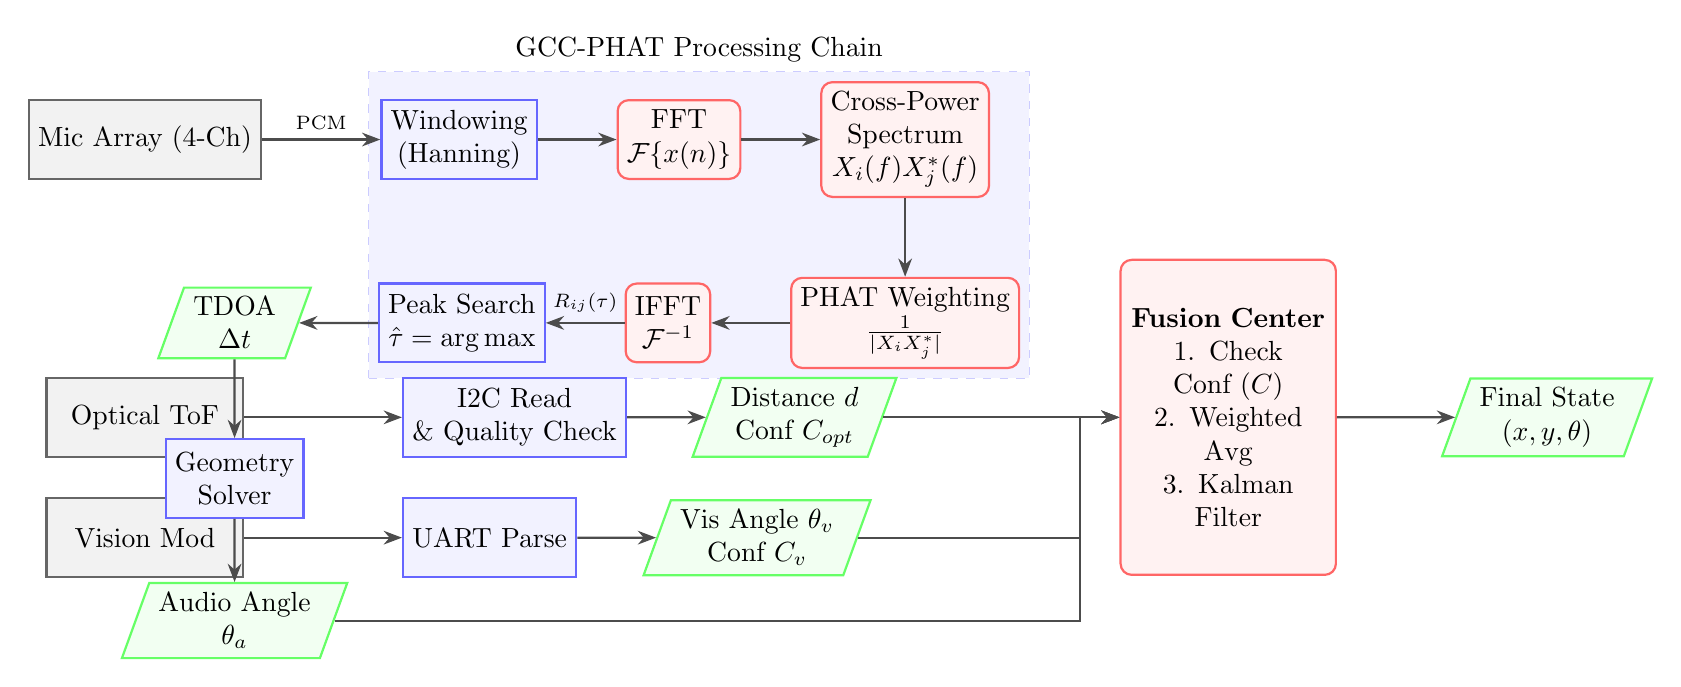
\begin{tikzpicture}[
    node distance=1.5cm and 1cm,
    >=Stealth,
    process/.style={rectangle, draw=blue!60, fill=blue!5, thick, minimum size=1cm, align=center},
    algo/.style={rectangle, rounded corners, draw=red!60, fill=red!5, thick, minimum size=1cm, align=center},
    data/.style={trapezium, trapezium left angle=70, trapezium right angle=110, draw=green!60, fill=green!5, thick, align=center},
    sensor/.style={rectangle, draw=black!60, fill=gray!10, thick, minimum width=2.5cm, minimum height=1cm},
    line/.style={->, thick, draw=black!70}
]

% 1. 输入源
\node[sensor] (mic) {Mic Array (4-Ch)};
\node[sensor, below=2.5cm of mic] (tof) {Optical ToF};
\node[sensor, below=0.5cm of tof] (cam) {Vision Mod};

% 2. 声学 DSP 链路 (Horizontal)
\node[process, right=1.5cm of mic] (window) {Windowing\\(Hanning)};
\node[algo, right=1cm of window] (fft) {FFT\\ $\mathcal{F}\{x(n)\}$};
\node[algo, right=1cm of fft] (cps) {Cross-Power\\ Spectrum\\ $X_i(f)X_j^*(f)$};
\node[algo, below=1cm of cps] (phat) {PHAT Weighting\\ $\frac{1}{|X_i X_j^*|}$};
\node[algo, left=1cm of phat] (ifft) {IFFT\\ $\mathcal{F}^{-1}$};
\node[process, left=1cm of ifft] (peak) {Peak Search\\ $\hat{\tau} = \arg\max$};
\node[data, left=1cm of peak] (tdoa) {TDOA\\ $\Delta t$};

% 3. 几何解算
\node[process, below=1cm of tdoa] (aoa) {Geometry\\ Solver};
\node[data, below=0.8cm of aoa] (angle_a) {Audio Angle\\ $\theta_a$};

% 4. 其他传感器链路
\node[process, right=2cm of tof] (read_tof) {I2C Read\\ \& Quality Check};
\node[data, right=1cm of read_tof] (dist) {Distance $d$\\ Conf $C_{opt}$};

\node[process, right=2cm of cam] (read_cam) {UART Parse};
\node[data, right=1cm of read_cam] (angle_v) {Vis Angle $\theta_v$\\ Conf $C_v$};

% 5. 融合中心
\node[algo, right=3cm of dist, minimum height=4cm, text width=2.5cm] (fusion) {
    \textbf{Fusion Center}\\
    1. Check Conf ($C$)\\
    2. Weighted Avg\\
    3. Kalman Filter
};

\node[data, right=1.5cm of fusion] (output) {Final State\\ $(x, y, \theta)$};

% 连线 - 声学
\draw[line] (mic) -- node[above, font=\scriptsize]{PCM} (window);
\draw[line] (window) -- (fft);
\draw[line] (fft) -- (cps);
\draw[line] (cps) -- (phat);
\draw[line] (phat) -- (ifft);
\draw[line] (ifft) -- node[above, font=\scriptsize]{$R_{ij}(\tau)$} (peak);
\draw[line] (peak) -- (tdoa);
\draw[line] (tdoa) -- (aoa);
\draw[line] (aoa) -- (angle_a);

% 连线 - 光学与视觉
\draw[line] (tof) -- (read_tof);
\draw[line] (read_tof) -- (dist);
\draw[line] (cam) -- (read_cam);
\draw[line] (read_cam) -- (angle_v);

% 连线 - 融合
\draw[line] (angle_a.east) -| ([xshift=-0.5cm]fusion.west) -- (fusion.west);
\draw[line] (dist.east) -- (fusion.west);
\draw[line] (angle_v.east) -| ([xshift=-0.5cm]fusion.west) -- (fusion.west);

\draw[line] (fusion) -- (output);

% 背景框
\begin{scope}[on background layer]
    \node[fit=(window)(fft)(cps)(phat)(ifft)(peak), fill=blue!5, draw=blue!20, dashed, label=above:GCC-PHAT Processing Chain] {};
\end{scope}

\end{tikzpicture}
\end{document}